\documentclass[]{book}
\usepackage{lmodern}
\usepackage{amssymb,amsmath}
\usepackage{ifxetex,ifluatex}
\usepackage{fixltx2e} % provides \textsubscript
\ifnum 0\ifxetex 1\fi\ifluatex 1\fi=0 % if pdftex
  \usepackage[T1]{fontenc}
  \usepackage[utf8]{inputenc}
\else % if luatex or xelatex
  \ifxetex
    \usepackage{mathspec}
  \else
    \usepackage{fontspec}
  \fi
  \defaultfontfeatures{Ligatures=TeX,Scale=MatchLowercase}
\fi
% use upquote if available, for straight quotes in verbatim environments
\IfFileExists{upquote.sty}{\usepackage{upquote}}{}
% use microtype if available
\IfFileExists{microtype.sty}{%
\usepackage{microtype}
\UseMicrotypeSet[protrusion]{basicmath} % disable protrusion for tt fonts
}{}
\usepackage[margin=1in]{geometry}
\usepackage{hyperref}
\hypersetup{unicode=true,
            pdftitle={Giới thiệu về Hệ phức hợp và Khoa học mạng lưới},
            pdfauthor={Nguyễn Quang},
            pdfborder={0 0 0},
            breaklinks=true}
\urlstyle{same}  % don't use monospace font for urls
\usepackage{natbib}
\bibliographystyle{apalike}
\usepackage{longtable,booktabs}
\usepackage{graphicx,grffile}
\makeatletter
\def\maxwidth{\ifdim\Gin@nat@width>\linewidth\linewidth\else\Gin@nat@width\fi}
\def\maxheight{\ifdim\Gin@nat@height>\textheight\textheight\else\Gin@nat@height\fi}
\makeatother
% Scale images if necessary, so that they will not overflow the page
% margins by default, and it is still possible to overwrite the defaults
% using explicit options in \includegraphics[width, height, ...]{}
\setkeys{Gin}{width=\maxwidth,height=\maxheight,keepaspectratio}
\IfFileExists{parskip.sty}{%
\usepackage{parskip}
}{% else
\setlength{\parindent}{0pt}
\setlength{\parskip}{6pt plus 2pt minus 1pt}
}
\setlength{\emergencystretch}{3em}  % prevent overfull lines
\providecommand{\tightlist}{%
  \setlength{\itemsep}{0pt}\setlength{\parskip}{0pt}}
\setcounter{secnumdepth}{5}
% Redefines (sub)paragraphs to behave more like sections
\ifx\paragraph\undefined\else
\let\oldparagraph\paragraph
\renewcommand{\paragraph}[1]{\oldparagraph{#1}\mbox{}}
\fi
\ifx\subparagraph\undefined\else
\let\oldsubparagraph\subparagraph
\renewcommand{\subparagraph}[1]{\oldsubparagraph{#1}\mbox{}}
\fi

%%% Use protect on footnotes to avoid problems with footnotes in titles
\let\rmarkdownfootnote\footnote%
\def\footnote{\protect\rmarkdownfootnote}

%%% Change title format to be more compact
\usepackage{titling}

% Create subtitle command for use in maketitle
\providecommand{\subtitle}[1]{
  \posttitle{
    \begin{center}\large#1\end{center}
    }
}

\setlength{\droptitle}{-2em}

  \title{Giới thiệu về Hệ phức hợp và Khoa học mạng lưới}
    \pretitle{\vspace{\droptitle}\centering\huge}
  \posttitle{\par}
    \author{Nguyễn Quang}
    \preauthor{\centering\large\emph}
  \postauthor{\par}
      \predate{\centering\large\emph}
  \postdate{\par}
    \date{2020-04-10}

\usepackage{booktabs}

\begin{document}
\maketitle

{
\setcounter{tocdepth}{1}
\tableofcontents
}
\chapter{Giới thiệu}\label{intro}

Stephen Hawking đã từng nói trong thế kỷ trước ``I think the next
{[}21st{]} century will be the century of complexity. We have already
discovered the basic laws{]} that govern matter and understand all the
normal situations. We don't know how the laws fit together, and what
happens under extreme conditions. But I expect we will find a complete
unified theory sometime this century. There is no limit to the
complexity that we can build using those basic laws.''
\href{https://en.wikiquote.org/wiki/Complexity}{nguồn} Tạm dịch là:

Tôi cho rằng thế kỷ tới (21) sẽ là thế kỷ của hệ phức hợp. Chúng ta đã
khám phá ra các định luật cơ bản chi phối vật chất và thông hiểu mọi
hiện tượng thông thường, nhưng lại không hiểu các định luật đó tương
thích với nhau như thế nào và điều gì sẽ xảy ra ở những thời điểm cực
điểm? Tôi kỳ vọng là chúng ta sẽ tìm ra một lý thuyết thống nhất hoàn
chỉnh trong thế kỷ tới. Với lý thuyết đó chúng ta có thể xây dựng những
thứ có độ phức tạp vô hạn.

Hệ phức hợp được định nghĩa là một hệ thống gồm \textbf{rất nhiều} phần
tử tương tác chặt chẽ với nhau, có tính chất tự tổ chức (self-organized)
và khả năng biến đổi tiến hóa (adapt) trong môi trường.

Thông thường các phần tử của hệ phức hợp có tính chất đơn giản. Chính sự
tương tác tạo ra tính ``phức hợp''" của nó. Do vậy, tính \textbf{rất
nhiều} phần tử là một đặc điểm tiên quyết bởi vi tính chất của một tập
hợp rất nhiều phần tử \textbf{không phải} bằng tổng tính chất của từng
phần tử đơn lẻ.

Có thể lấy ví dụ về hệ phức hợp như hệ sinh thái, một nền kinh tế, mạng
Internet, mạng xã hội, mạng truyền tải điện, mạng giao thông, hệ địa
chất, hệ miễn dịch trong cơ thể, bộ não sinh học, một đàn kiến đông,
virut lan truyền trong xã hội, hệ thời tiết, \ldots{}

\begin{figure}

{\centering 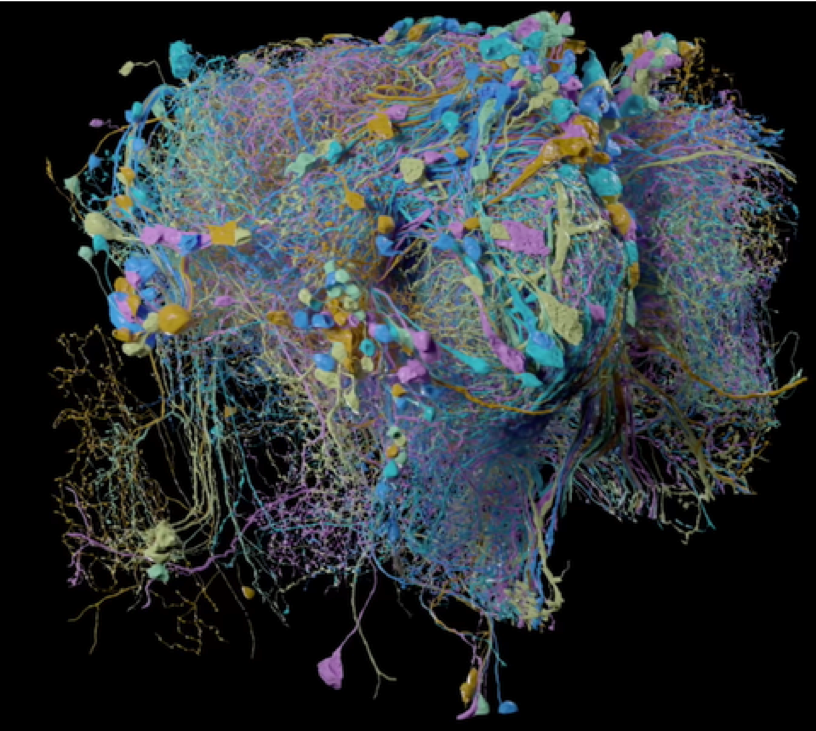
\includegraphics[width=0.5\linewidth]{images/flybrain} 

}

\caption{Bộ não con ruồi với 25,000 neuron và 25 triệu dây thần kinh là một hệ phức hợp - nguồn: Google}\label{fig:flybrain}
\end{figure}\begin{figure}

{\centering 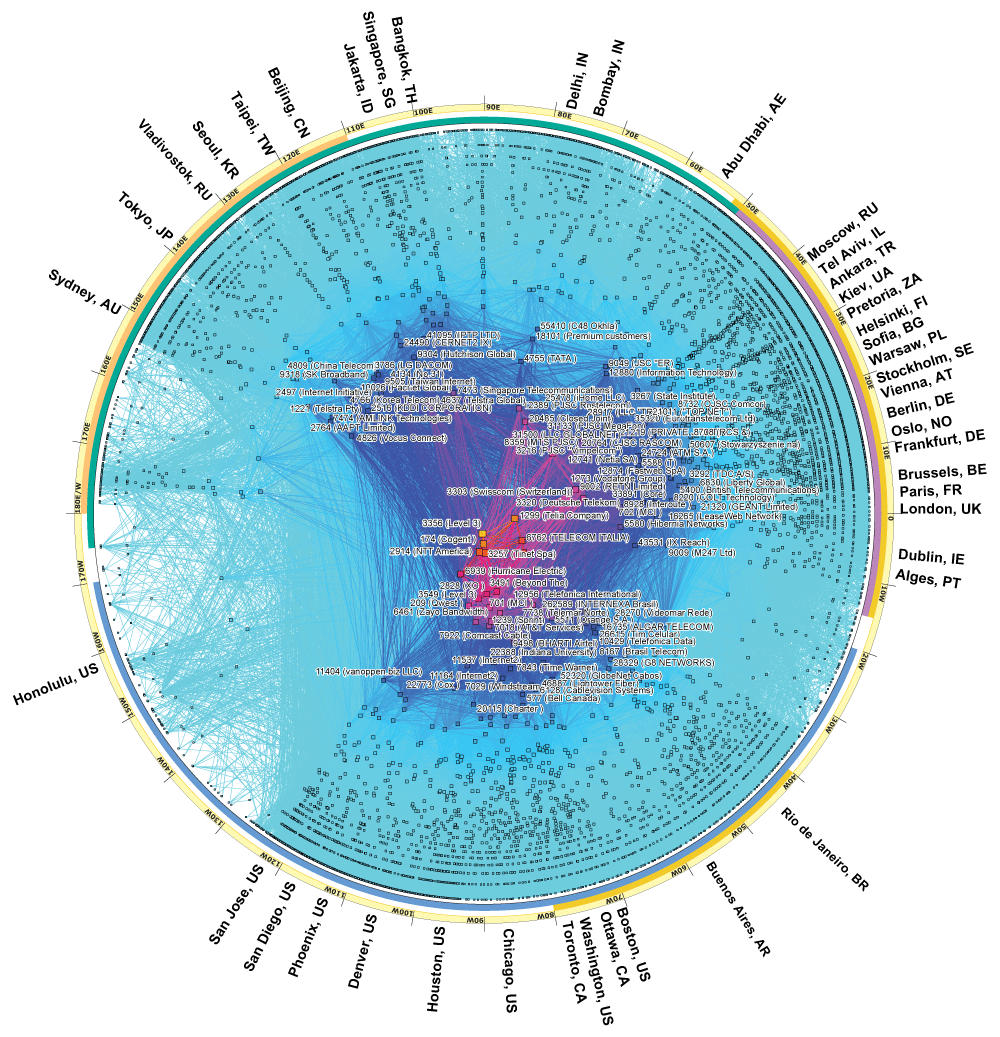
\includegraphics[width=0.5\linewidth]{images/internet2020} 

}

\caption{Mạng Internet IPv4 có 47,610 Autonomous Systems' (ASes) và 148,455 kết nối là một hệ phức hợp - nguồn: caida.org}\label{fig:internet}
\end{figure}

\section{Các tính chất của hệ phức hợp}\label{cac-tinh-cht-cua-h-phc-hp}

Sự vận hành các hệ phức hợp có những tính chất đặc biệt như:

\begin{itemize}
\item
  \textbf{Tính tiến hóa}: các phần tử của hệ khi tương tác với các phần
  tử khác có thể thay đổi hành vi của mình và thích ứng với môi trường.
\item
  \textbf{Tính đột phát} (emergence): hệ có thể xuất hiện những hình
  dạng/cấu trúc và hành vi mới mà không thể đoán được nếu chỉ dựa trên
  các định luật cơ bản của phần tử thành phần hoặc chính.
\item
  \textbf{Tính tự tổ chức}: khi biến đổi thích ứng, các phần tử có thể
  tương tác và hệ tự diễn biến về một trạng thái dừng (mà không cần bộ
  phận điều khiển trung tâm).
\item
  \textbf{Điểm hút}: là những trạng thái mà hệ có thể tiến hóa đến mặc
  dù điều kiện ban đầu của thời điểm tiến hóa khác nhau.
\item
  \textbf{Tính tự tổ chức quan trọng}: (self-organized criticality): có
  một số điểm hút mà hệ tự tiến hóa về và dừng lại, sau đó hệ diễn biến
  rất đột ngột với cường độ trải dài trong một khoảng rộng và
  \textbf{không đoán được}. Về dài hạn thì cường độ này tuân theo một
  phân bố phổ biến là luật hàm mũ.
\item
  \textbf{Tính hỗn loạn}(chaos): là những biến đổi không dự đoán được và
  rất nhạy cảm với điều kiện ban đầu. Sự hỗn loạn này thường không kiểm
  soát được và phải mất một thời gian hệ mới ổn định lại. (Nhiều khi hệ
  phức hợp được hiểu nhầm là hệ hỗn loạn - chaotic system - dù hệ phức
  hợp có tính chất rộng hơn)
\item
  \textbf{Tính phi tuyến}: rất nhiều biến đổi của hệ có tính phi tuyến
  và để dự báo được cần nhiều các thuật toán phi tuyến phức tạp và ứng
  dụng của xác suất.
\item
  \textbf{Sự chuyển pha}: Tính tự tổ chức quan trọng là điểm xảy ra sự
  chuyển pha. Sự chuyển pha này thường diễn ra đột ngột, cường độ mạnh
  và có thể là quá trình không đảo ngược được. (Sự chuyển pha trong các
  hệ tự nhiên đã được nghiên cứu nhiều như nước đá tan thành
  nước,\ldots{} và có thể vận dụng các kiến thức này nhưng sự chuyển pha
  trong các hệ phức hợp phức tạp hơn).
\end{itemize}

Bảng sau đây đưa ra một vài ví dụ về một số tính chất của ba hệ phức hợp
tiêu biểu: mạng Internet (cần phân biệt với mạng WWW), một nền kinh tế
và một bộ não sinh học.

\begin{tabu} to \linewidth {>{\raggedright}X>{\raggedright}X>{\raggedright}X>{\raggedright}X}
\hline
Network & Adaptable & Emergence & Chaos\\
\hline
Mạng Internet & Sự phát triển và mở rộng mạng phù hợp với địa lý và nhu cầu liên lạc & Sự lan truyền thông tin có thể gây nghẽn mạng & Các nút/router có thể bị ngắt đồng thời trên diện rộng và không kiểm soát\\
\hline
Nền kinh tế & Sự phát triển kinh tế thỏa mãn các nhu cầu tiêu dùng của con người & Khủng hoảng xuất hiện sau một thời gian phát triển tốt đẹp & Cung/cầu đổi chiều liên tục trong một thời gian ngắn\\
\hline
Bộ não sinh học & Các kết nối dây thần kinh thay đổi phù hợp với sự tiến hóa & Các phát minh bột phát sau qua trình suy nghĩ & Mất trí nhớ\\
\hline
\end{tabu}

\section{Khoa học Hệ phức hợp (Complex
sicence)}\label{khoa-hoc-h-phc-hp-complex-sicence}

Chính vì sự phổ biến và quan trọng của các hệ phức hợp, Khoa học hệ phức
hợp (``Complex Science'') đang trở thành một hướng quan trọng và thu hút
sự chú ý của các nhà nghiên cứu và xã hội. Đây là một hướng nghiên cứu
đa ngành với các định luật có thể đến từ Vật lý thống kê, Toán học, Lý
thuyết thông tin, Hệ động lực, \ldots{} nhưng cũng có thể đến từ nhiều
ngành ứng dụng như Kinh tế học, Sinh học, Xã hội học,\ldots{} Trong 22
chương trình (sáng kiến) KHCN của lộ trình tới 2050 của Trung Quốc, có 4
sáng kiến về ``nghiên cứu cơ bản'' và 3 sáng kiến về ``nghiên cứu liên
ngành và tiên tiến'', trong đó Hệ phức hợp là một hướng nghiên cứu liên
ngành trọng tâm*.

Nghiên cứu về Hệ phức hợp có thể chia thành hai nhánh nhỏ hơn:

\begin{itemize}
\item
  Nghiên cứu về \textbf{cấu trúc} của hệ: thành phần, liên kết, phân bố
  tính chất, tính phân nhóm, sự biến đổi cấu trúc theo thời gian, hệ
  siêu lớn, biểu diễn hình ảnh,\ldots{}
\item
  Nghiên cứu về \textbf{quá trình động lực} (dynamic process) diễn ra
  trong hệ: quá trình tan rã, phá vỡ, chuyển pha; quá trình lan truyền
  thông thông/dịch bệnh và điều khiển ngăn chặn; các quá trình chuyển
  pha và đột phát, mô phỏng và dự báo,\ldots{}
\end{itemize}

Hai nhánh này có thể kết hợp và bổ sung cho nhau: Hiểu cấu trúc sẽ mô tả
tốt hơn các quá trình diễn ra trên hệ.

Các nghiên cứu này nếu được thực hiện sẽ đóng góp quan trọng cho nghiên
cứu cơ bản và ứng dụng ví dụ như:

\begin{itemize}
\item
  Tăng cường sự ổn định và phòng ngừa khả năng đổ vỡ dây chuyền của các
  hệ như Internet, mạng lưới truyền tải điện, mạng lưới giao
  thông,\ldots{}
\item
  Hiểu rõ và điều khiển các quá trình lan truyền (thông tin, dịch
  bệnh,\ldots{})
\item
  Dự báo xã hội (khủng hoảng kinh tế) và đề xuất các chính sách ổn định
\item
  Phát triển các thuật toán AI dựa trên sự hiểu biết về các tương tác
  giữa nơron trong não bộ, tiến đến trí thông minh tiến hóa.
\item
  Phát triển các máy AI hoặc cấu trúc máy tính mới dựa trên các cấu trúc
  Vật lý hoàn toàn mới.
\item
  Hỗ trợ các phát minh sinh học và y tế dựa trên sự hiểu biết về tương
  tác trong các hệ vi sinh \ldots{}
\end{itemize}

\section{Các phương pháp nghiên cứu
chính:}\label{cac-phuong-phap-nghien-cu-chinh}

Hiện nay có hai phương pháp tiếp cận nghiên cứu chính đối với hệ phức
hợp là:

\begin{enumerate}
\def\labelenumi{\arabic{enumi}.}
\tightlist
\item
  \textbf{Mô phỏng đa tác nhân} (``Agent-based modeling''): đây là cách
  tiếp cận dạng ``bottom-up'' bằng cách mô phỏng số lượng lớn các tác
  nhân có tính chất và hành vi của hệ thực cần nghiên cứu. Kết quả mô
  phỏng sẽ cho ra một hệ ảo và có thể xác định được cấu trúc, hoặc tiếp
  tục sử dụng để mô phỏng các quá trình động học trong hệ.
\end{enumerate}

Hướng nghiên cứu này có lợi điểm là mô phỏng được số lượng lớn tác nhân,
mô phỏng hệ có quan hệ phức tạp,\ldots{} nhưng có nhược điểm là thiếu
các lý thuyết, mô hình hỗ trợ

\begin{enumerate}
\def\labelenumi{\arabic{enumi}.}
\setcounter{enumi}{1}
\tightlist
\item
  \textbf{Khoa học mạng lưới} (``Network Science''): một điều dễ dàng là
  hầu hết các hệ phức hợp có thể được mô tả bởi một mạng lưới, hay một
  đồ thị trong ngôn ngữ Toán học.
\end{enumerate}

Cách tiếp cận này có thể tận dụng được các lý thuyết và mô hình từ lý
thuyết đồ thị, vật lý thống kê,\ldots{} Các mô hình được xây dựng từ đơn
giản đến phức tạp nên có tính hệ thống hơn.

Ví dụ về hình ảnh của mạng lưới 500 sân bay lớn trên nước Mỹ:

\begin{figure}

{\centering 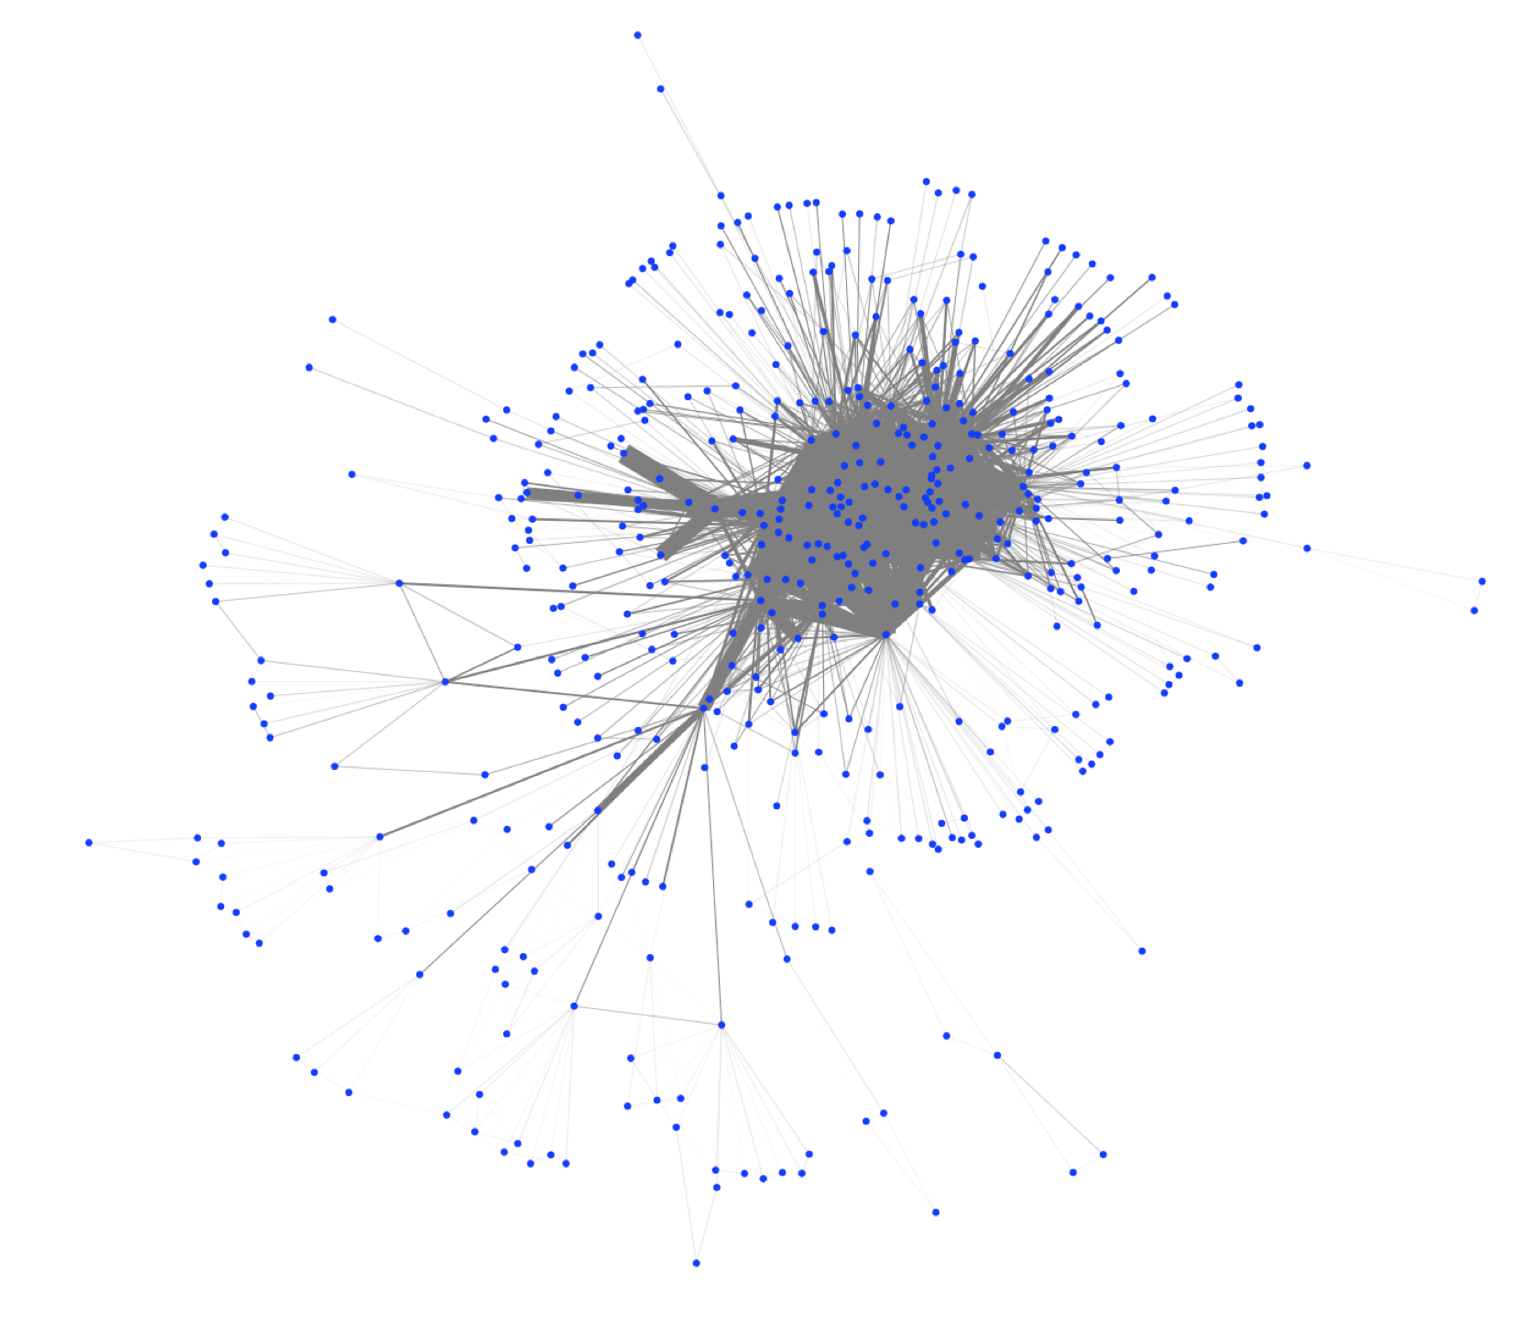
\includegraphics[width=1\linewidth]{images/US_500airports} 

}

\caption{Mạng lưới 500 sân bay thương mại lớn nhất của nước Mỹ - nguồn dữ liệu: (Dall’Asta et al. 2006)}\label{fig:USairport}
\end{figure}

Trong tài liệu này tôi sẽ tập trung vào hướng khoa học mạng lưới nhiều
hơn là mô phỏng đa tác nhân.

\subsection{Tham khảo:}\label{tham-khao}

Albert-Laszlo Barabasi. Linked. The New Science of Networks. Perseus
Publ., 2002

M.E.J. Newman. Networks. An Introduction. Oxford Univ. Press, 2010

Mitchell, Melanie, Complexity: A Guided Tour Oxford University Press:
New York, NY, 2009

Dall'Asta, Luca, Alain Barrat, Marc Barthélemy, and Alessandro
Vespignani. 2006. ``Vulnerability of Weighted Networks.'' Journal of
Statistical Mechanics: Theory and Experiment.

\begin{itemize}
\tightlist
\item
  Theo thầy Nguyễn Ái Việt
  \href{https://www.facebook.com/aiviet.nguyen.9?__tn__=\%2CdC-R-R\&eid=ARAJ1vCKX01Y4m8vomc-RQMwqgoWWzWqDudM8pAkDrbitzWK5jUOfzJL7H-fi3lD-TLvTmejQqrdrGNC\&hc_ref=ARTz8R9ntR0lsAhLWBjxkYsdR-84qhnvs4OSnd3F4WtMzfNjOk7-lgkzYbfHYRJiXVk\&fref=nf}{tổng
  hợp} lại.
\end{itemize}

\chapter{Giới thiệu về khoa học mạng lưới}\label{intro}

\section{Các định nghĩa cơ bản}\label{cac-inh-nghia-co-ban}

\subsection{Định nghĩa mạng lưới}\label{inh-nghia-mang-lui}

Một mạng lưới là một đồ thị toán học ký hiệu bởi \(G = G(E,V)\) bao gồm:
- Một tập hợp các đỉnh (``vertex/node'') \(V\) - Một tập hợp các cạnh
(``edge/link''): \(E\) gồm những cặp đỉnh trong \(V\)

Ví dụ sau biểu diễn một đồ thị gồm 5 đỉnh và 7 cạnh:

\begin{itemize}
\item
  \(V = {1, 2, 3, 4, 5}\)
\item
  \(E = {(1, 2), (2, 3), (3, 1), (3, 4)}\)
  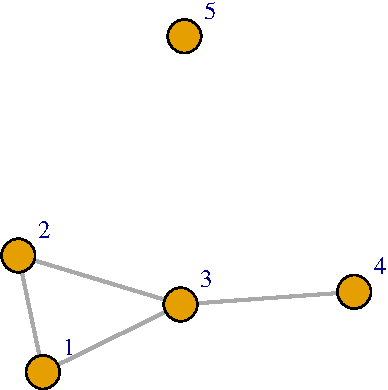
\includegraphics{ComplexNetwork_files/figure-latex/graph1-1.pdf}
\end{itemize}

Các đỉnh thường được ký hiệu bởi số nguyên từ \(1\) đến \(n\):
\(1,2,...,n\). Tập hợp cạnh \(E\) còn được gọi là danh sách cạnh.

Có thể biểu diễn mạng lưới theo một cách khác là ma trận kề \(A\) có
chiều \(n \times n\). Như với đồ thị trên chúng ta có:

\begin{Bmatrix}
    0 & 1 & 1 & 0 & 0 \\
    1 & 0 & 1 & 0 & 0 \\
    1 & 1 & 0 & 1 & 0 \\
    0 & 0 & 1 & 0 & 0 \\
    0 & 0 & 0 & 0 & 0 \\
\end{Bmatrix}

Với các giá trị \(a_{ij}\) bằng 1 nếu có tồn tại một cạnh giữa \(i\) và
\(j\) và bằng 0 nếu không.

\begin{itemize}
\item
  Mạng lưới có thể có hướng (``directed''), khi đó cạnh \((i,j)\) được
  coi là đi từ đỉnh \(i\) tới đỉnh \(j\), nếu không thì gọi là không
  hướng.
\item
  Có thể có cạnh đi từ một đỉnh tới chính nó (``self-edge'').
\item
  Có thể có nhiều cạnh giữa 2 đỉnh (``multiedges''), khi đó giá trị
  \(a_{ij}\) là số nguyên bằng số cạnh giữa 2 đỉnh.
\item
  Một nhóm mạng lưới quan trọng khác là \textbf{mạng có trong số}
  (``weighted network''). Khi đó mỗi cạnh đều có một giá trị không âm và
  các giá trị \(a_{ij}\) của ma trận kề có cùng giá trị với trọng số
  tương ứng của cạnh.
\item
  Mạng lưới có tồn tại cạnh nối 2 đỉnh bất kỳ gọi là \textbf{mạng đầy
  đủ} (``complete graph'')
\end{itemize}

\section{Các phép đo lường cơ bản}\label{cac-phep-o-lung-co-ban}

Dựa trên cấu trúc mạng lưới chúng ta có thể tính toán các phép đo cho
đỉnh, cạnh hay toàn mạng lưới.

\subsection{Bậc và phân phối bậc}\label{bc-va-phan-phi-bc}

Bậc (``degree'') của một đỉnh \(i\), ký hiệu \(k_i\), là tổng số cạnh đi
tới nó. Với một mạng không hướng thì có thể tính bậc mỗi đỉnh bởi tổng
của hàng \(i\) tương ứng của ma trận kề \(A\):
\(k_i = \sum_{j = 1}^{n}a_{ij}\).

Cũng với mạng không hướng, nếu có \(m\) cạnh thì tổng số bậc của tất cả
các đỉnh sẽ là \(2m\). Ví dụ như với mạng 500 sân bay lớn nhất của Mỹ
trong hình \eqref{eq:USairport} ta có các thông số sau:

\begin{table}[H]
\centering
\begin{tabular}{>{\bfseries}l||r}
\hline
Measure & Value\\
\hline
Số đỉnh & 500.00\\
\hline
Số cạnh & 2980.00\\
\hline
Bậc TB & 5.96\\
\hline
\end{tabular}
\end{table}

Như vậy một sân bay trung bình chỉ có gần 6 đường bay nội địa? Con số
trung bình này không phản ánh rõ bởi ở Mỹ có rất nhiều sân bay nhỏ chỉ
kết nối với một vài sân bay chính gần đó. Có đến 74 sân bay chỉ kết nối
duy nhất 1 sân bay khác (trong số 500 sân bay lớn), 107 sân bay kết nối
với 2 sân bay khác, và sân bay kết nối nhiều nhất có 146 đường bay khác
nhau, như thể hiện qua đồ thị tần số (histogram) dưới đây.

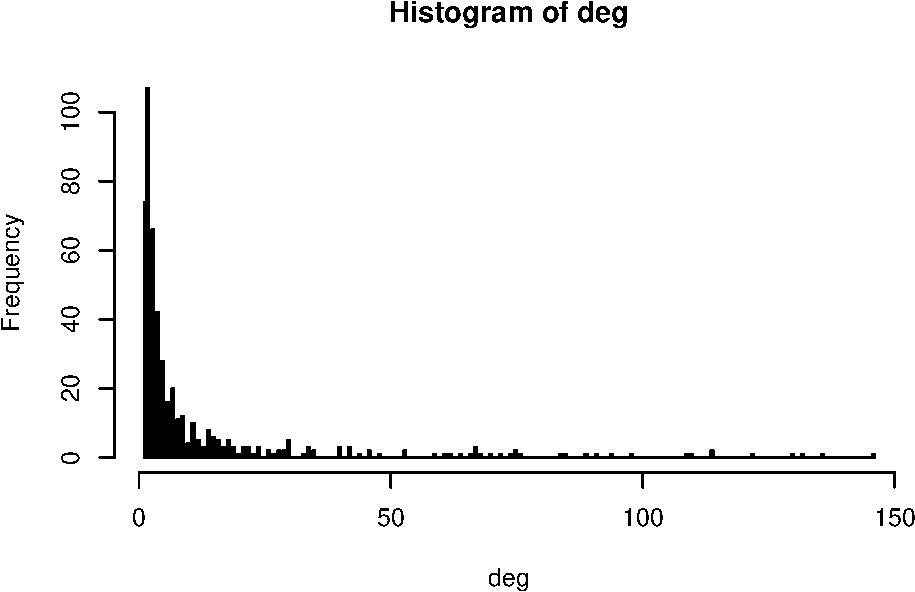
\includegraphics{ComplexNetwork_files/figure-latex/unnamed-chunk-3-1.pdf}

Chúng ta có thể thấy các mạng thực tế thường có phân bố bậc rất rộng và
không đối xứng, với rất nhiều đỉnh có số bậc nhỏ và một số ít đỉnh có số
bậc rất lớn. Các dữ liệu thực nghiệm cho thấy phần lớn các phân phối này
có dạng hàm mũ ở phần đuôi, với số mũ từ thông thường từ 2-3.

\begin{figure}

{\centering 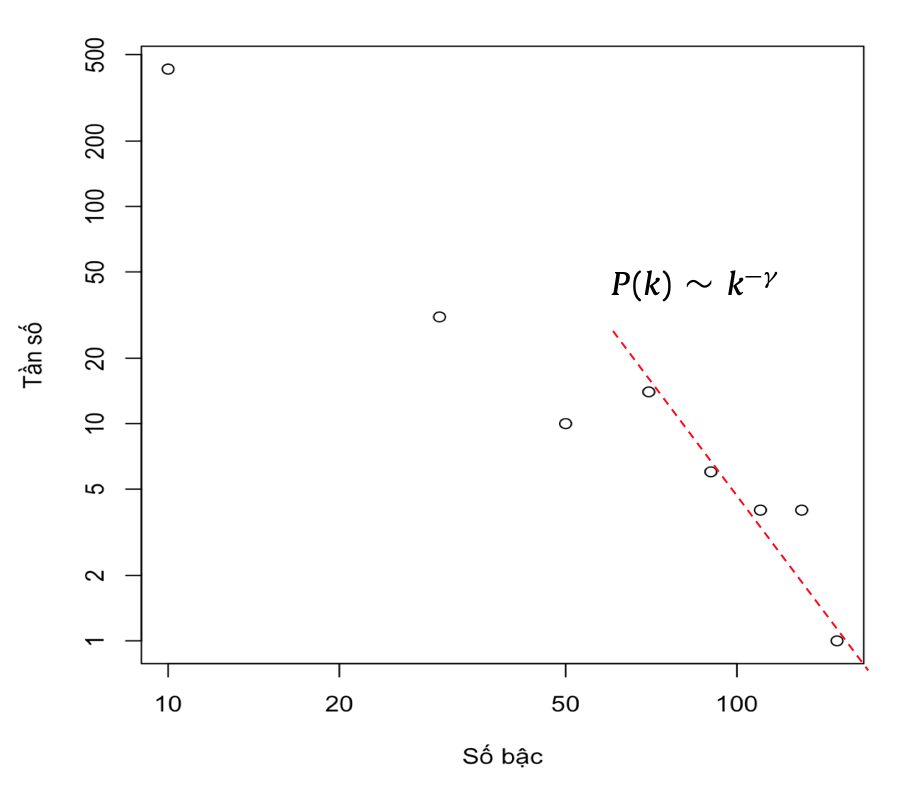
\includegraphics[width=0.8\linewidth]{images/USAirport_500_deg} 

}

\caption{Bậc của mạng 500 sân bay tuân theo phân bố hàm mũ (phần đuôi) giống như nhiều mạng lưới thực tế khác}(\#fig:USAirport_500_deg)
\end{figure}

\subsection{Đường đi và đường đi ngắn
nhất}\label{ung-i-va-ung-i-ngn-nht}

Đường đi (``path'') giữa hai đỉnh \(i\) và \(j\) là tập hợp các cạnh nối
từ \(i\) tới \(j\). Giữa hai đỉnh bất kỳ có thể không tồn tại đường đi,
hoặc tồn tại nhiều đường đi.

Ví dụ về một đường đi ngắn nhất giữa 2 sân bay (màu đỏ) là 2 cạnh màu
xanh nước biển, đi qua một sân bay khác màu xanh lá cây:

\begin{figure}
\centering
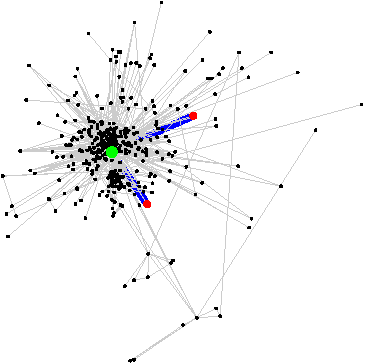
\includegraphics{ComplexNetwork_files/figure-latex/unnamed-chunk-5-1.pdf}
\caption{\label{fig:unnamed-chunk-5}Ví dụ về một đường đi ngắn nhất giữa 2
sân bay (màu đỏ), trung chuyển qua một sân bay khác (màu xanh)}
\end{figure}

\begin{itemize}
\tightlist
\item
  \textbf{Đường đi ngắn nhất trung bình} là trung bình của mọi đường đi
  ngăn nhất giữa hai đỉnh (nếu có). Đây là một phép đo quan trọng thể
  hiện sự kết nối. Với mạng 500 sân bay Mỹ là 2.9896902 hay gần 3, có
  nghĩa là trung bình để đi từ hai sân bay bất kỳ trên đất Mỹ cần đi 3
  chuyến bay.
\end{itemize}

Một hiện tượng nổi tiếng ``Six degrees of separation'' phát hiện bởi
Frigyes Karinthy, viết lại bởi John Guare chỉ ra hai người bất kỳ trong
xã hội có thể kết nối với nhau chỉ qua trung bình 6 người trung gian
khác (xem
\href{https://en.wikipedia.org/wiki/Six_degrees_of_separation}{Wikipedia}).
Đây là một con số nhỏ ngạc nhiên vào thời trước, và được mô tả thành
hiện tượng \textbf{thế giới nhỏ} (``the small-world effect'').

\begin{itemize}
\item
  \textbf{chiều} của mạng lưới là giá trị lớn nhất của tất cả các đường
  đi ngắn nhất. Với mạng 500 sân bay Mỹ là 7.
\item
  Mạng lưới mà luôn tồn tại ít nhất một đường đi giữa hai đỉnh bất kỳ
  gọi là \textbf{mạng kết nối}.
\item
  Một mạng lưới không kết nối có thể chia thành nhiều mạng kết nối rời
  rạc với nhau. Các mạng con kết nối này được gọi là các \textbf{thành
  phần} (``components'') của mạng ban đầu.
\item
  Thành phần có kích thước lớn nhất của một mạng lưới gọi là
  \textbf{LCC} (``Largest connected components''). (Với mạng kết nối thì
  LCC chính là mạng lưới)
\end{itemize}

\subsection{Tính trung gian}\label{tinh-trung-gian}

Dựa trên đường đi ngăn nhất, tính trung gian (``betweenness'') của một
đỉnh \(i\), \(b_i\) là tổng số đường đi ngăn nhất giữa hai đỉnh khác
\(i\) mà đi qua \(i\). Tính trung gian là một phép đo rất quan trọng của
mỗi đỉnh. Đỉnh có tính trung gian cao thường đóng vai trò kết nối cao
trong một mạng lưới.

Với mạng có trọng số, mỗi đường đi ngắn nhất được tính theo trong số và
tính trung gian trọng số là tổng giá trị của các đường đi ngắn nhất đi
qua đỉnh.

\section{Tính phân nhóm}\label{tinh-phan-nhom}

Ngoài các tính chất đã kể trên của mạng lưới là 1) phân bố bậc dạng hàm
mũ và 2) tính chất ``small-world'', các mạng thực tế thường có sự phân
nhóm ít nhiều khác nhau, đặc biệt là các mạng xã hội.

Xác định nhóm trong mạng là một trong những bài toán quan trọng và có
nhiều cách tiếp cận khác nhau. Tính phân nhóm ảnh hưởng quan trọng đến
các quá trình động lực sau này của mạng lưới.

\section{Các mô hình mạng lưới cơ
bản}\label{cac-mo-hinh-mang-lui-co-ban}

\chapter{Tính bền vững của mạng lưới}\label{tinh-bn-vng-cua-mang-lui}

Tính bền vững của mạng lưới (``Network Roburstness/Resilience'') là một
đối tượng nghiên cứu đầu tiên trong nhánh các quá trình động lực.

\chapter{Các mô hình lan truyền và phòng ngừa dịch
bệnh}\label{cac-mo-hinh-lan-truyn-va-phong-nga-dich-bnh}

\section{Các mô hình lan truyền}\label{cac-mo-hinh-lan-truyn}

\subsection{Mô hình lan truyền cổ điển:}\label{mo-hinh-lan-truyn-c-in}

Mô hình lan truyền được Kermack và McKendrick {[}1{]} phát triển đầu
tiên vào năm 1927, dựa trên lý thuyết trường trung bình động (dynamic
mean-field theory). Giả thuyết cơ bản của mô hình này là mỗi cá nhân
tương tác với tất cả các cá nhân khác trong xã hội một cách ngẫu nhiên
giống nhau. Xác suất nhiễm bệnh, khỏi bệnh,\ldots{} của mỗi cá nhân là
giống nhau và tỷ lệ với tỷ lệ trung bình chung của xã hội. Chi tiết của
mô hình này có thể tìm đọc trên
\href{https://en.wikipedia.org/wiki/Mathematical_modelling_of_infectious_disease}{Wikipedia}
hoặc trong
\href{http://vinif.org/vi/khoa-hoc-thuong-thuc/read/1/mo-hinh-du-bao-ngan-han-va-dai-han-kha-nang-lan-rong-cua-dich-2019-ncov-tu-vu-han-o-pham-vi-trung-quoc-va-quoc-te}{bài
viết} của TS. Hoàng Ngọc Thạch và TS. Phan Thị Hà Dương (VinIF) với các
tham số cập nhật cho dịch bệnh Covid-19. Ở đây tôi tóm lược một số kết
quả chính của mô hình cổ điển như sau:

Một tập hợp N (cố định) cá nhân/người dân có thể ở trong một số trạng
thái xác định là: + Có khả năng mắc bệnh (\textbf{S}usceptible) + Nhiễm
bệnh và có thể lây cho người khác (\textbf{I}nfected) + Không còn khả
năng mắc bệnh (\textbf{R}emoved hay Recovered - đã chữa khỏi hoặc đã
chết).

Có thể mô phỏng quá trình chuyển đổi trạng thái theo nhiều cách, trong
đó 2 mô hình phổ biến nhất là: * SIS:

\begin{itemize}
\tightlist
\item
  Một cá nhân từ \textbf{S} có thể bị nhiễm bệnh và chuyển sang
  \textbf{I} với xác suất \(\alpha\) trong một đơn vị thời gian tỷ lệ
  với tỷ lệ nhiễm bệnh hiện tại: \(\alpha = \beta\frac{I}{N}\),
\end{itemize}

trong đó \(I\) là số người bị nhiễm hiện tại và \(\beta\) gọi là tỷ lệ
nhiễm bệnh (infection rate). Phương trình này áp dụng như nhau cho mỗi
cá nhân và dựa trên giả thuyết mỗi cá nhân tiếp xúc với tất cả mọi người
trong xã hội với xác suất như nhau.

\begin{itemize}
\tightlist
\item
  Một cá nhân từ \textbf{I} có thể được chữa khỏi và chuyển sang
  \textbf{S} với xác suất \(\mu\) trong một đơn vị thời gian, với giả
  thuyết việc chữa bệnh được áp dụng như nhau cho mọi người bệnh.
\end{itemize}

Kết hợp lại chúng ta có thể mô tả quá trình động lực của số nhiễm bệnh
(\textbf{I}) và khỏe mạnh (\textbf{S}) bằng các phương trình vi phân xác
định như sau :

\begin{equation} 
  \frac{dI}{dt} = S\times\beta \frac{I}{N}-\mu I
  \label{eq:SIS1}
\end{equation}

\begin{equation} 
  \frac{dS}{dt} = -I\times\beta \frac{S}{N}+\mu I
  \label{eq:SIS2}
\end{equation}

Phương trình \eqref{eq:SIS1} và \eqref{eq:SIS2} có thể hiểu là xác suất một
người khỏe bị nhiễm bệnh \(I/S\) bằng \(\beta\) nhân tỷ lệ nhiễm trung
bình trong cộng đồng. Xác suất một người nhiễm khỏi bệnh \(S/I\) bằng
\(\mu\)

(mặc dù các quá trình \(S -> I -> S\) là ngẫu nhiên nhưng cách tiếp cận
trên cho phép rút gọn lại thành phương trình xác định)

Một thông số quan trọng là một người bệnh làm lây nhiễm thêm cho bao
nhiêu người trong một đơn vị thời gian có thể biểu diễn là:

\begin{equation*} 
  R = \frac{dI^*}{Idt} = \beta \frac{S}{N}
  \label{eq:SIS2}
\end{equation*}

trong đó \(I^*\) là số lây nhiễm mới.

Trong giai đoạn đầu của dịch bệnh khi \(S\approx N\) thì các phương
trình có thể được rút gọn xấp xỉ và ta có thể định nghĩa
\(R_0 = \frac{\beta}{\mu}\) gọi là Hệ số lây nhiễm cơ bản. Đây là số ca
nhiễm F1 gây ra bởi một ca nhiễm F0 trong cộng đồng trong một đơn vị
thời gian. Kết quả chính của hệ phương trình là:

\begin{itemize}
\tightlist
\item
  Nếu \(R_0 > 1\) thì dịch bệnh sẽ bùng phát
\item
  Nếu \(R_0 < 1\) thì dịch bệnh sẽ tự tiêu biến
\item
  Nếu \(R_0 = 1\) thì dịch bệnh ở trạng thái dừng đặc hữu (endemic). Với
  số bệnh là hằng số mà không cần tác động
\end{itemize}

Ở Việt Nam hiện nay một số bệnh nhân F0 có thể tiếp xúc lên đến
\textbf{hơn 200 lần}. Giả sử trung bình các bệnh nhân F0 tiếp xúc 30
người trước khi bị phát hiện và nếu tỷ lệ nhiễm bệnh chỉ là 10\% thì
\(\beta = 30* 10\% = 3\). Với giá trị \(\mu < 1\) thì \(R_0 > 3\) và
nguy cơ gây ra bùng phát là rất cao.

Kết quả giải hệ phương trình trên cho toàn bộ quá trình động lực như
sau:

\begin{figure}

{\centering 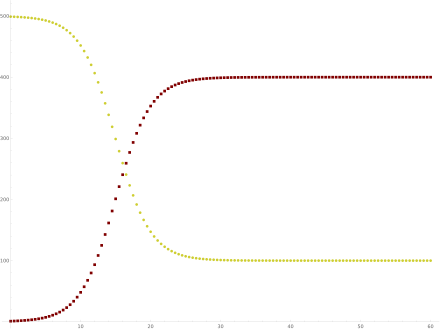
\includegraphics[width=0.5\linewidth]{images/SIS} 

}

\caption{Kết quả giải hệ SIS - nguồn: Wikipedia}\label{fig:SIS}
\end{figure}

\begin{itemize}
\tightlist
\item
  SIR: một cá nhân từ \textbf{S} có thể bị nhiễm bệnh và chuyển sang
  \textbf{I} và một cá nhân từ \textbf{I} có thể được chữa khỏi (và
  không thể lây nhiễm tiếp) hoặc chết đi và chuyển sang \textbf{R}. Cơ
  chế tương tự như SIS trong đó phân biệt rõ hơn trạng thái \textbf{R}.
  (Trong SIS thì \textbf{R} ẩn trong \textbf{S}). Dưới đây là kết quả
  giải hệ SIR từ nguồn
  \href{https://en.wikipedia.org/wiki/Compartmental_models_in_epidemiology}{Wikipedia}
\end{itemize}

\begin{figure}

{\centering 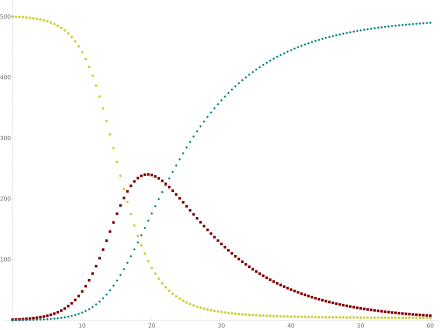
\includegraphics[width=0.5\linewidth]{images/SIR} 

}

\caption{Kết quả giải hệ SIR - nguồn: Wikipedia}\label{fig:SIR}
\end{figure}

Nhìn chung, kết quả từ các mô hình cổ điển SIS và SIR cho thấy trong
giai đoạn đầu, tỷ lệ nhiễm (cho SIS) và chết (cho SIR) sẽ tăng theo hàm
mũ và đạt ngưỡng bão hòa sau một thời gian. Ngưỡng này thường sẽ rất cao
lên đến nhiều chục \% trong dân số. Ở đó số lượng người khỏe còn quá ít
nên số lượng nhiễm mới bằng số lượng khỏi (\(\beta\ S = \mu I\)) hay còn
gọi là \textbf{miễn dịch cộng đồng}.

\subsection{Mô hình lan truyền theo mạng
lưới:}\label{mo-hinh-lan-truyn-theo-mang-lui}

Các giả thuyết rằng mỗi cá nhân giống nhau và giao tiếp ngẫu nhiên đều
trong toàn xã hội của các mô hình cổ điển là khá đơn giản. Trên thực tế,
mỗi người có mạng lưới tương tác xã hội của riêng mình. Phần lớn các cá
nhận chỉ tương tác với một số lượng hạn chế người khác, trong khi đó có
một phần nhỏ cá nhân tương tác với rất nhiều người khác. Dựa trên mô
hình mạng lưới, Diekmann {[}2{]} cho rằng Hệ số lây nhiễm cơ bản \(R_0\)
cần phải điều chính tính đến cấu trúc của mạng lưới tương tác.

\begin{figure}

{\centering 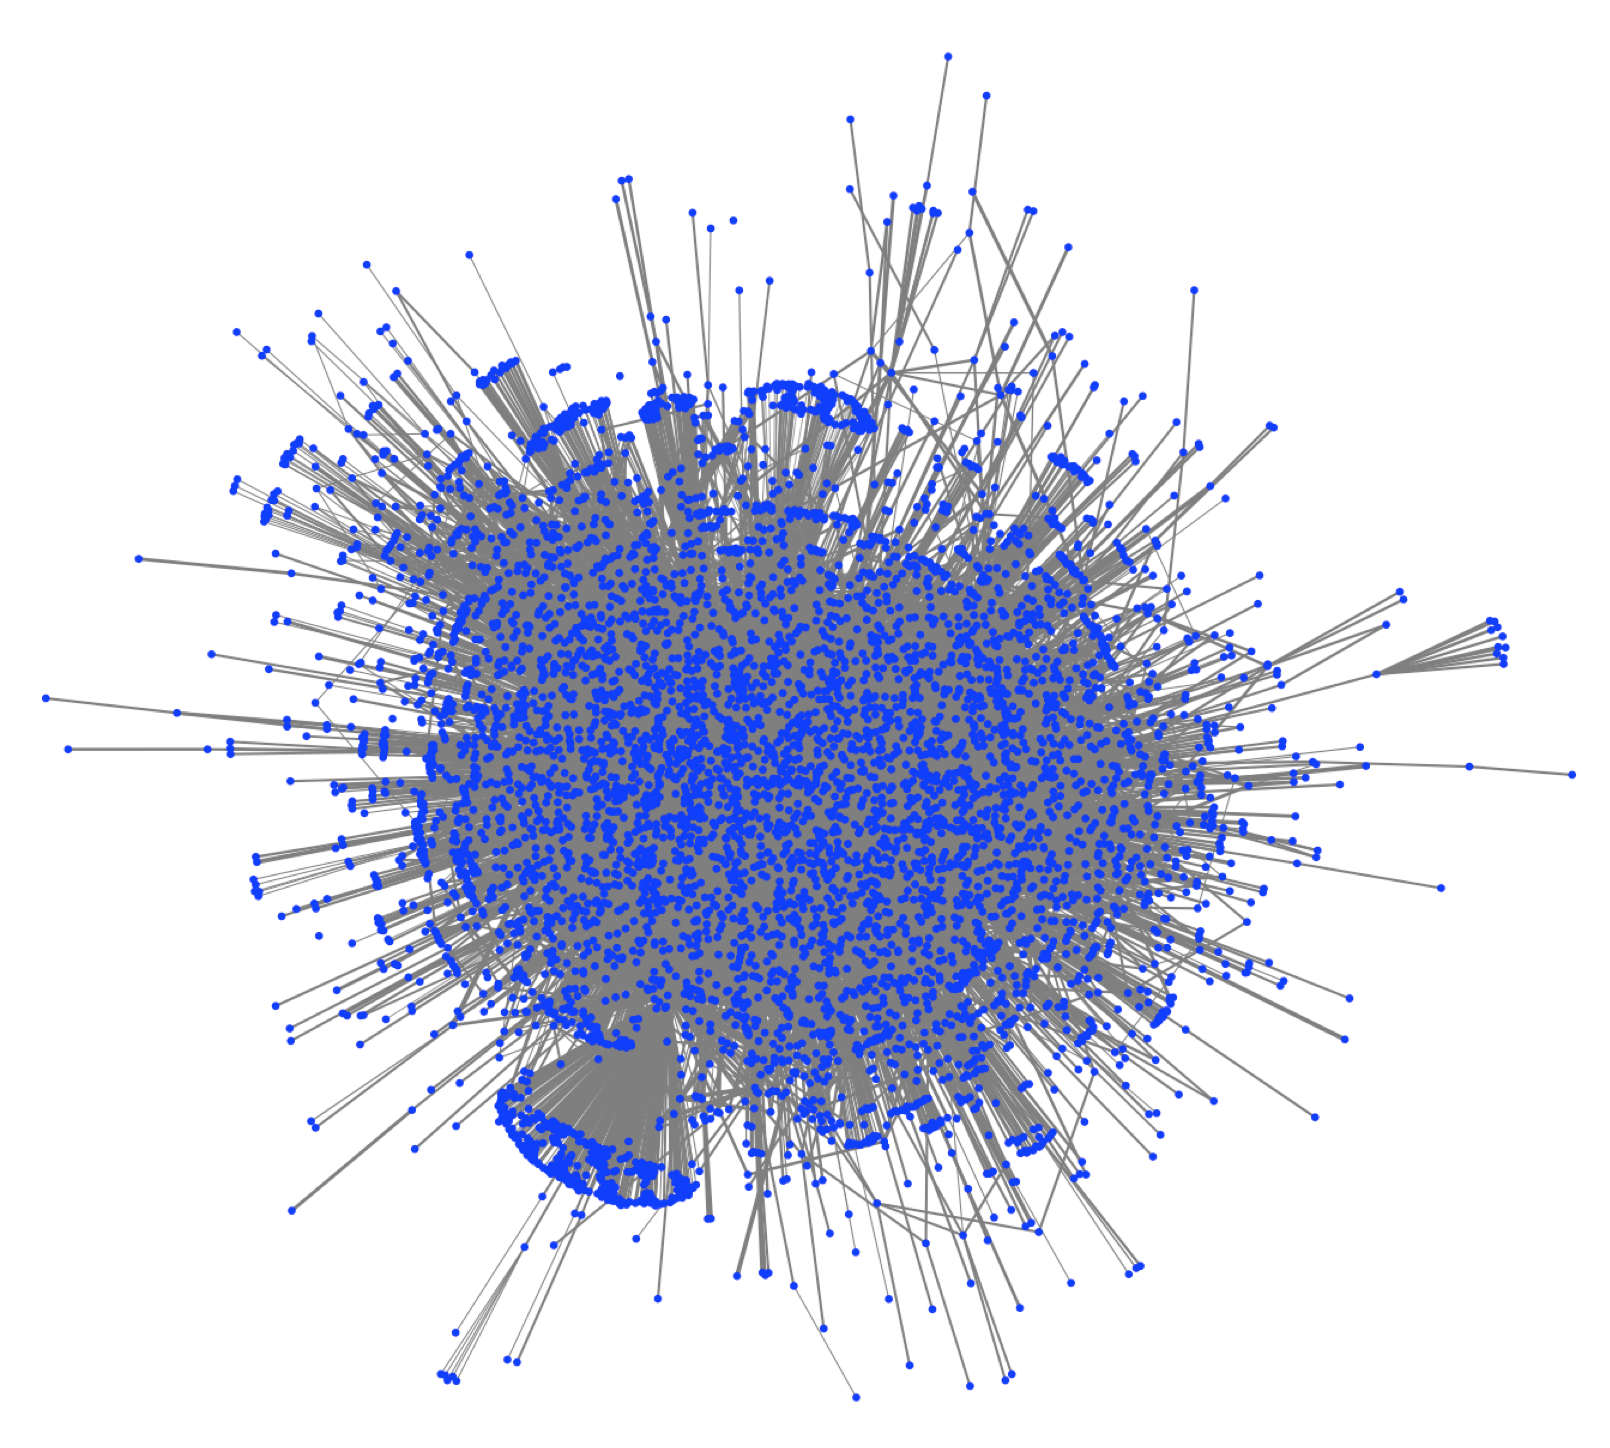
\includegraphics[width=0.8\linewidth]{images/bitcoin_LCC} 

}

\caption{Hình ảnh mô tả một mạng lưới tương tác xã hội - nguồn: tác giả}\label{fig:network1}
\end{figure}

Mạng lưới tương tác xã hội cũng giống như nhiều mạng lưới phức hợp khác
(``complex networks'') với nhiều đặc trưng riêng biệt, trong đó các quan
trọng nhất về cấu trúc là:

\begin{itemize}
\tightlist
\item
  Tính phân bố bậc: Bậc k - hay số tương tác của mỗi cá nhân - thường
  phân bố theo dạng hàm mũ, phản ánh tính khác biệt về sự tương tác rất
  lớn: một số cá nhân nhỏ tương tác với rất nhiều cá nhân khác trong khi
  phần lớn các cá nhân chỉ tương tác với một số nhỏ cá nhân khác.
\end{itemize}

\begin{figure}

{\centering 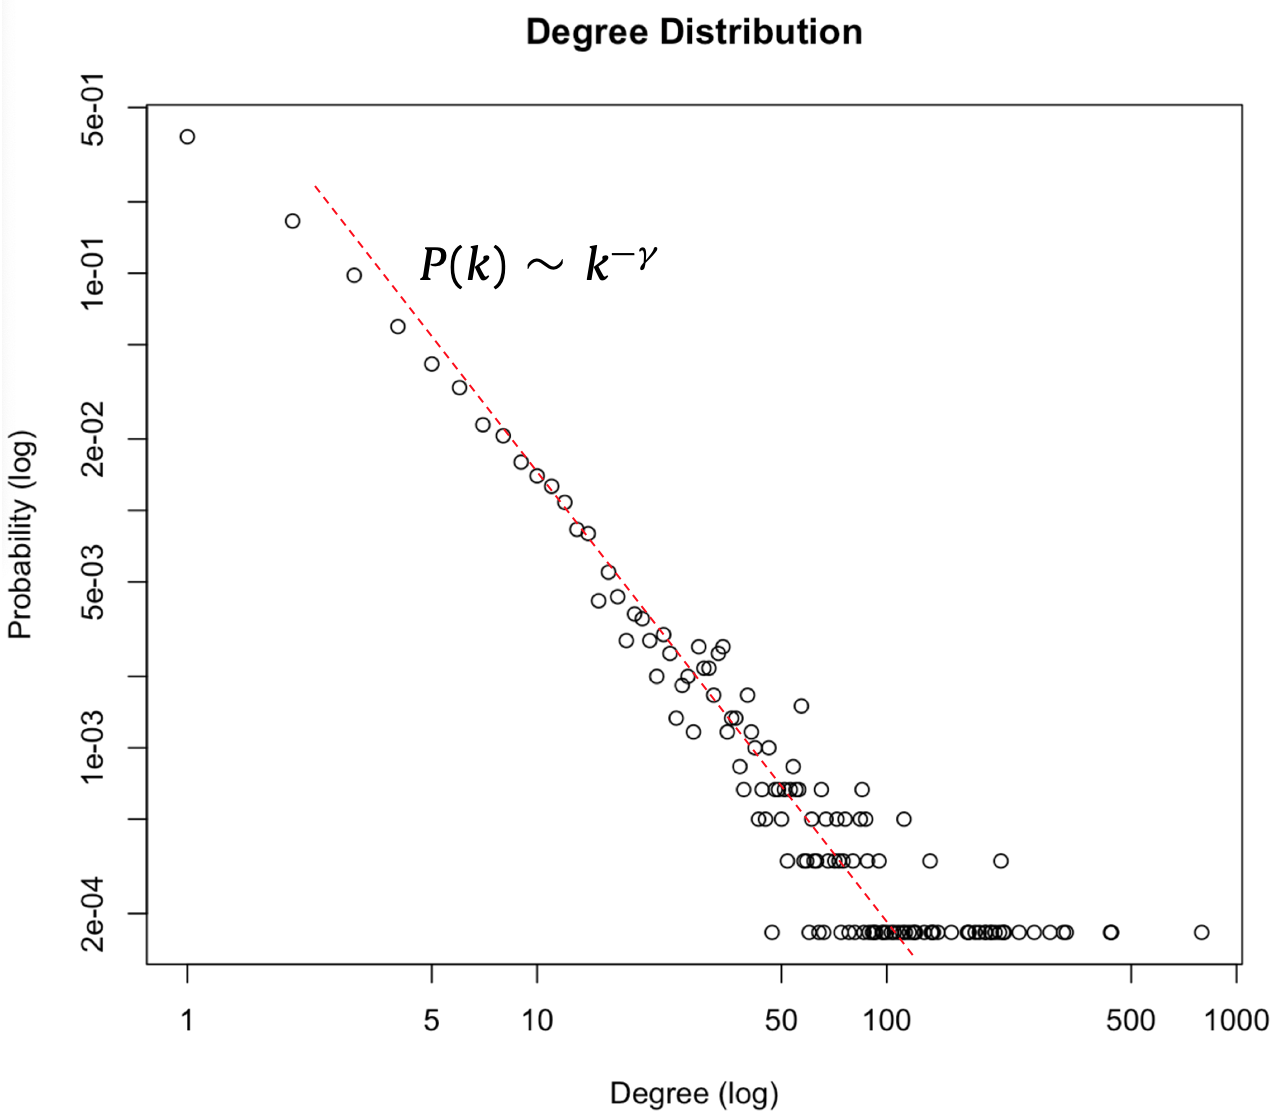
\includegraphics[width=0.5\linewidth]{images/bitcoin_degree_dist_2} 

}

\caption{Phân phối bậc của các cá nhân trong mạng lưới trên - nguồn: tác giả}\label{fig:network1dist}
\end{figure}

\begin{itemize}
\tightlist
\item
  Tính phân nhóm: Mạng tương tác xã hội thường phân cụm thành những nhóm
  riêng biệt. Phần lớn các cá nhân chỉ tương tác với những cá nhân trong
  cùng một nhóm, một phần nhỏ các cá nhân tương tác với những cá nhân
  trong nhiều nhóm khác nhau. Các các nhân này mang tính liên kết rất
  cao và có thể, nhưng không nhất thiết, là các cá nhân có bậc cao hoặc
  rất cao.
\end{itemize}

\begin{figure}

{\centering 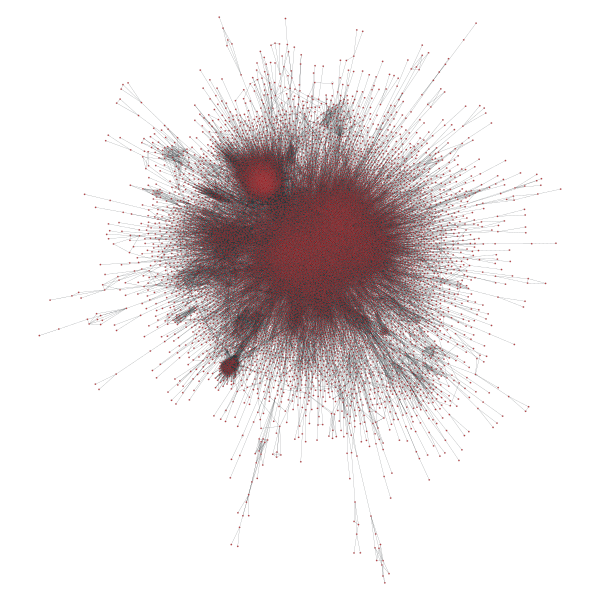
\includegraphics[width=0.6\linewidth]{images/public-figure} 

}

\caption{Một mạng lưới xã hội với tính phân nhóm cao - nguồn: [3]}\label{fig:network2}
\end{figure}

Một trong những phát triển đầu tiên của mô hình này do Pastor-Satorras
and Vespignani (2001) đề xuất {[}4{]}, kế thừa trên lý thuyết trường
trung bình động nhưng xét sự khác nhau của các cá nhân theo số bậc tương
tác k, gọi là ``degree-based mean-field theory'' (DBMF). Theo đó, các cá
nhân được mô tả khác nhau theo số tương tác k mà họ có, và phương trình
\eqref{eq:SIS1} được viết lại như sau cho mỗi giá trị bậc k:

\begin{equation} 
  \frac{dI_k}{dt} = \beta k [1-I_k]\sum_{k'} P[k'|k]\times \frac{I_{k'}}{N} -\mu I_k
  \label{eq:DBMF1}
\end{equation}

Dựa theo biểu thức đầu tiên của vế phải phương trình trên ta thấy một cá
nhân khỏe có bậc k có thể bị nhiễm với xác suất là tích của:

\begin{itemize}
\item
  k: số tương tác anh ta có
\item
  Tổng của \(P[k'|k]\): Xác suất anh ta có liên kết với một cá nhân có
  bậc k' khác và \(\frac{I_{k'}}{N}\): Tỷ lệ cá nhân có bậc k' bị nhiễm
\end{itemize}

Dựa trên cấu trúc của mạng lưới chúng ta có thể ước lượng \(P[k'|k]\) và
giải hệ trên một cách xấp xỉ bởi phương pháp phân tích trung bình tuyến
tính {[}6{]} (lời giải chính xác không khả thi). Kết quả chính của mô
hình này là điều kiện xảy ra bùng phát dịch (điểm tới hạn) nếu:

\(R_0 = \frac{\beta}{\mu} > \frac{<k>}{<k^2>}\)

(\(<>\) là ký hiệu của kỳ vọng, giả thiết các nút không tương quan
(uncorrelated network)).

Trong hình vẽ 4.3 tôi lấy ví dụ một mạng xã hội nhỏ gồm 6005 nút. Các dữ
liệu về tương tác xã hội thực không hoàn toàn giống mạng xã hội và không
sẵn có, do vậy kết quả có thể khác nhiều. Với mạng lưới trên ta có thể
tính các thông số mạng là:

\begin{itemize}
\item
  \(<k> = 7.15\)
\item
  \(<k^2> = 79\)
\item
  \(\frac{<k>}{<k^2>} = 0.012\)
\end{itemize}

Giả sử tỷ lệ chữa khỏi \(\mu = 0.4\) thì xác suất nhiễm bệnh khi tiếp
xúc \(\beta\) cần phải dưới giá trị
\(\mu\frac{<k>}{<k^2>} = 0.4*0.012 \approx 0.5\%\) và rất không khả thi.

Trong trường hợp cách ly các tương tác (nói rõ hơn trong phần sau) chúng
ta sẽ có được mạng lưới mới với số cạnh tối thiểu:

\begin{figure}

{\centering 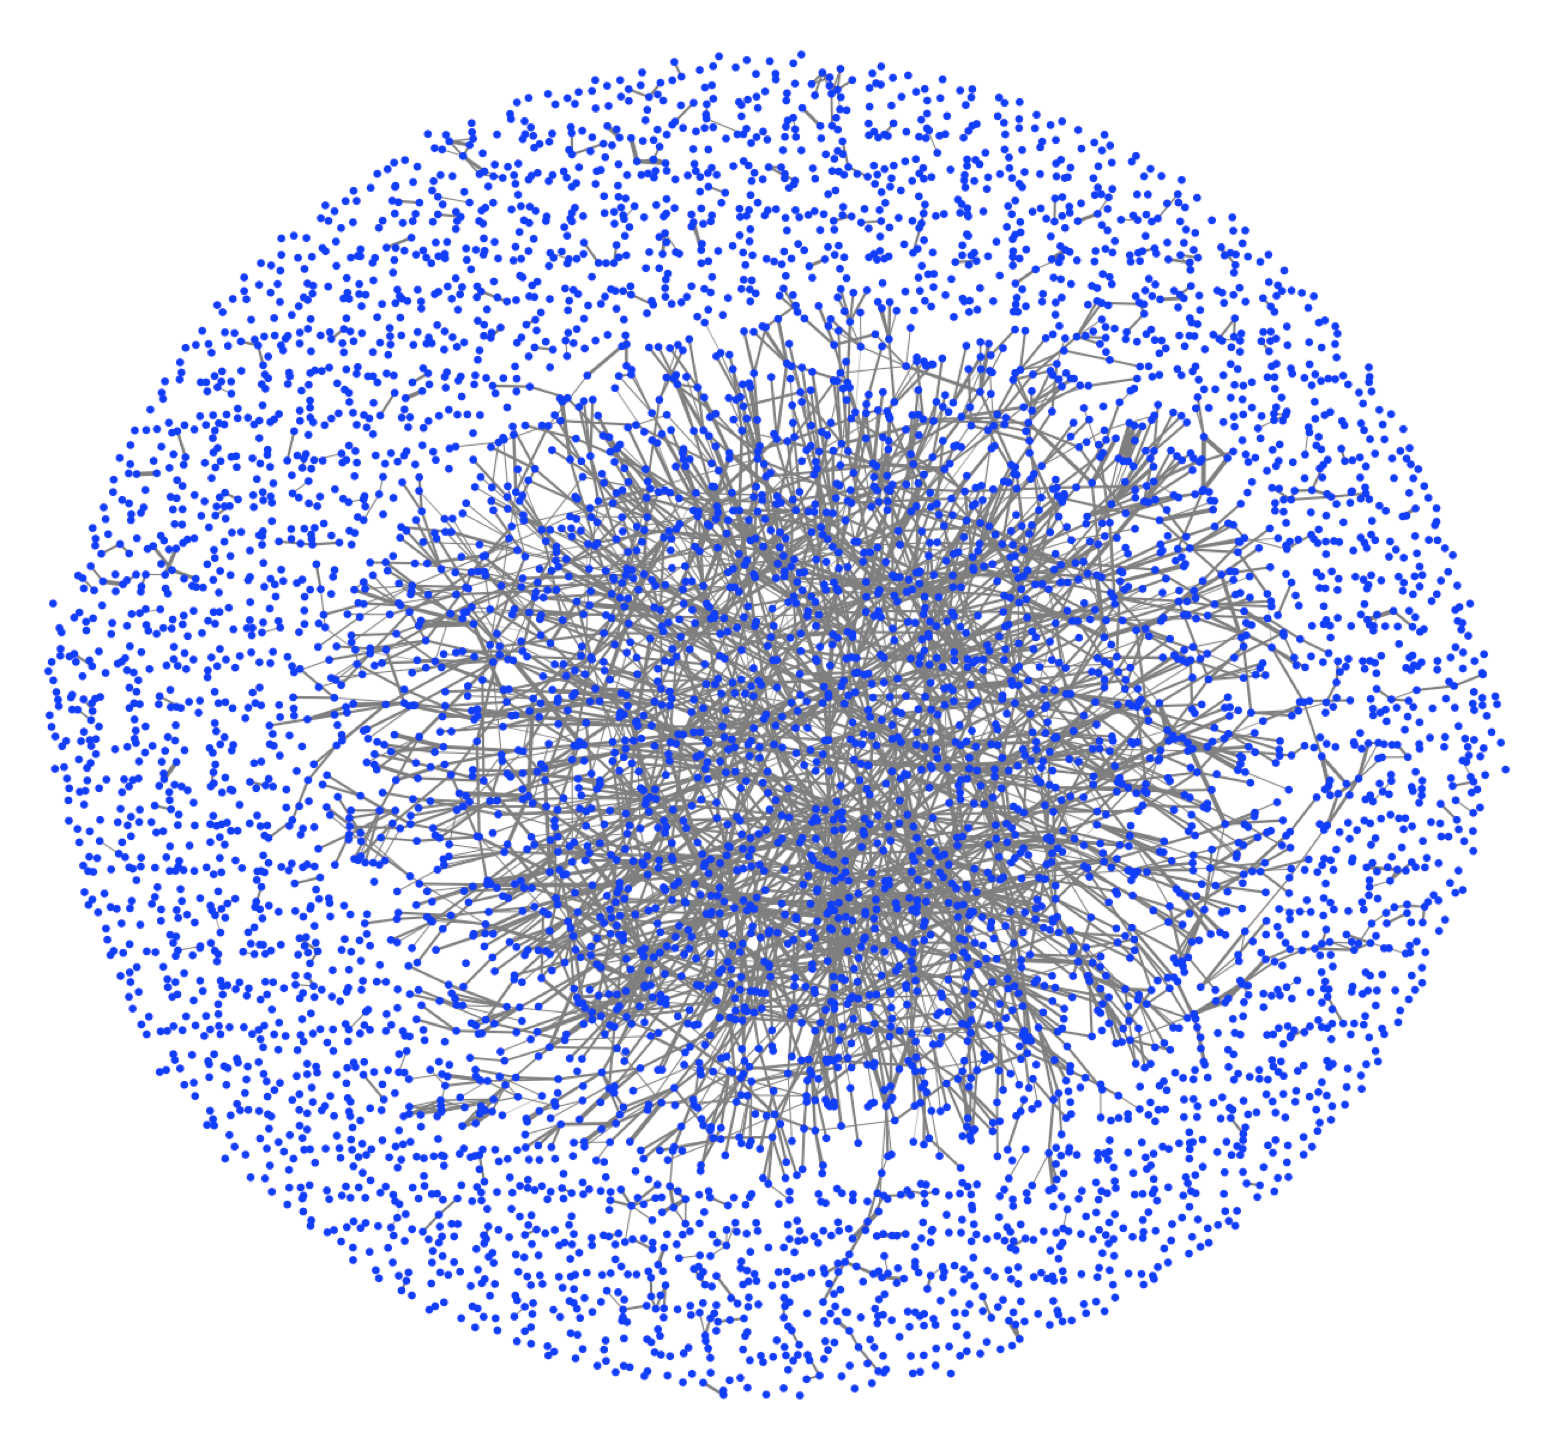
\includegraphics[width=0.8\linewidth]{images/bitcoin_delete_edges} 

}

\caption{Một mạng lưới xã hội với tính phân nhóm cao - nguồn: [3]}\label{fig:network3}
\end{figure}

Khi đó các thông số mạng trở thành:

\begin{itemize}
\item
  \(<k> = 1.27\)
\item
  \(<k^2> = 3.45\)
\item
  \(\frac{<k>}{<k^2>} = 0.289\)
\end{itemize}

Giả sử tỷ lệ chữa khỏi \(\mu = 0.4\) thì xác suất nhiễm bệnh khi tiếp
xúc \(\beta\) cần phải dưới giá trị
\(\mu\frac{<k>}{<k^2>} = 0.4*0.289 \approx 11.5\%\). Xác suất này dễ đạt
được hơn và cao hơn ngưỡng trước khi cách ly hơn 20 lần.

\subsection{Các phương pháp mô phỏng:}\label{cac-phuong-phap-mo-phong}

Việc xây dựng các mô hình gần với thực tế hơn thường sẽ khiến cho các
phương trình trở nên phức tạp và rất khó giải. Khi đó các phương pháp mô
phỏng sẽ trở nên đặc biệt hữu ích. Ví dụ với một dữ liệu mạng lưới cho
trước chúng ta có thể ước lượng xác suất bùng phát dịch bằng cách cho
lan truyền giả định lặp lại nhiều lần, với rất nhiều tham số khác nhau.
(to be continued)

\section{Các mô hình phòng ngừa}\label{cac-mo-hinh-phong-nga}

Các mô hình trong phần trên giả định việc lan truyền tự nhiên và không
có tác động từ bên ngoài. Trong thực tế, chúng ta luôn mong muốn ngăn
chặn số người bị nhiễm bệnh và tác động vào việc lan truyền. Các mô hình
phòng ngừa được đặt ra nhằm tối ưu hiệu quả của tác động hoặc giảm thiểu
chi phí cho một mục tiêu xác định. (to be continued)

\subsection{Mô hình tiêm ngừa (immunization
model)}\label{mo-hinh-tiem-nga-immunization-model}

Trong trường hợp đã có vaccin phòng bệnh thì tiêm chủng mở rộng là biện
pháp an toàn nhất (nếu có thể). Đây chính là các chương trình tiêm chủng
cho mọi trẻ em đã được áp dụng. Ở một số nơi khác như các nước châu Phi,
số lượng vaccin có ít nên các mô hình immunization có thể được sử dụng
để xác định ra đối tượng vaccin có hiệu quả nhất trong việc ngăn ngừa
lan truyền trong cộng đồng. (to be continued)

\subsection{Mô hình cách ly xã hội}\label{mo-hinh-cach-ly-xa-hi}

Trong trường hợp chưa có vaccin phòng bệnh thì biện pháp chính là dùng
các dụng cụ bảo hộ tối đa (tiếp xúc nhưng giảm thiểu xác suất lây
nhiễm), tương ứng việc giảm hệ số \(\beta\) ban đầu, hoặc trong trường
hợp bất khả kháng (không xác định được ai đang nhiễm và sẽ nhiễm cho ai)
thì phá vỡ mạng lưới tương tác xã hội (cách ly) là biện pháp cuối cùng.
Cách phá vỡ mạng lưới có thể bao gồm: + Phá vỡ nút (cá nhân) bằng cách
ly tập trung + Phá vỡ cạnh (phá vỡ tương tác) bằng cách ly xã hội

\section{Tham khảo:}\label{tham-khao-1}

{[}1{]} W. O. Kermack and A. G. McKendrick, Contributions to the
mathematical theory of epidemics part I, Proc. R. Soc. Edinb., A115,
700--721, 1927.

{[}2{]} Diekmann, O., H. Heesterbeek, and T. Britton (2012), Math-
ematical Tools for Understanding Infectious Disease Dy- namics
(Princeton University Press, Princeton, USA).

{[}3{]} Quang Nguyen, Hanh-Duyen Dinh , Thi-Trang Le , Thanh-Trung
Nguyen , Michele Bellingeri, ``Structure and Robustness of Facebook's
pages networks'' (Applied Network Science - accepted)

{[}4{]} Pastor-Satorras, R., and A. Vespignani (2001b), Phys. Rev.~Lett.
86, 3200.

{[}5{]} Romualdo Pastor-Satorras, Claudio Castellano, Piet Van Mieghem,
Alessandro Vespignani, ``Epidemic processes in complex networks''.
Review of Modern Physics 87(3) 2014

{[}6{]} Bogun ̃a ́, M., and R. Pastor-Satorras (2002), Phys. Rev.~E 66,
047104.

\chapter{Applications}\label{applications}

Some \emph{significant} applications are demonstrated in this chapter.

\section{Example one}\label{example-one}

\section{Example two}\label{example-two}

\chapter{Final Words}\label{final-words}

We have finished a nice book.

\bibliography{book.bib,packages.bib}


\end{document}
